\documentclass{beamer}
\usepackage{graphicx}
\usepackage[utf8]{inputenc}
\usepackage[T1]{fontenc} % avec T1 comme option  d'encodage c'est ben mieux, surtout pour taper du français.

\usetheme[hideallsubsections]{PaloAlto}

\usepackage{tikz}
\usepackage{verbatim}
\usepackage{tabularx}
\usepackage{array}

% centre verticlament le texte pour les colonnes en X
\renewcommand{\tabularxcolumn}[1]{>{\small}m{#1}}
\usepackage{makecell}
\usepackage{color}
\usepackage{diagbox}

\usepackage[french,english]{babel}
\usepackage{lmodern} % fortement conseillé pour les pdf. On peut mettre autre chose : kpfonts, fourier,...


% \setbeamertemplate{sections in toc}[sections numbered]
% \usetikzlibrary{arrows,shadows,shapes,backgrounds,positioning}
% \beamertemplatetransparentcovered

% insert page number in Beamer Navigation Bars
\addtobeamertemplate{navigation symbols}{}{%
    \usebeamerfont{footline}%
    \usebeamercolor[fg]{footline}%
    \hspace{1em}%
    \insertframenumber/\inserttotalframenumber
}

% set head height
\makeatletter
\setlength{\beamer@headheight}{0.7cm}
\makeatother


\title[]{Gestion des licences d'un projet informatique} 
\author{Rémi Boulle  \href{mailto:mail@remiboulle.fr}{mail@remiboulle.fr}}
\date{}       
\institute{}        

\begin{document}

% Titre des sections dans une slide dédiée
\AtBeginSection[]{
  \begin{frame}
  \vfill
  \centering
  \begin{beamercolorbox}[sep=8pt,center,shadow=true,rounded=true]{title}
    \usebeamerfont{title}\insertsectionhead\par%
  \end{beamercolorbox}
  \vfill
  \end{frame}
}

%%%%%%%%%%%%%%%%
% Titre
%%%%%%%%%%%%%%%%

\begin{frame}
  \titlepage
\end{frame}


%\section{Objectifs}

\begin{frame}
\frametitle{Objectif g\'en\'eral}
\begin{alertblock}{Objectif}
  Acquérir/renforcer expertise sur les licences logicielles libres
\end{alertblock}


  \begin{itemize}
  \item Historique et contexte
  \item Différentes catégories de licences
  \item Règles de diffusivité et compatibilité
  \item Outils d'audits pour de gros projets
  \item Économie du logiciel
  \end{itemize}
\end{frame}

%%%%%%%%%%%%%%%%%%%%%%%%%%%%%%%%%%%%%%%%%%%%%%%%%%%%%%%%
% Contexte et historique
%%%%%%%%%%%%%%%%%%%%%%%%%%%%%%%%%%%%%%%%%%%%%%%%%%%%%%%%

\section{Contexte}

\begin{frame}{Historique}
  \begin{itemize}
  \item projet GNU en 1984 par Richard Stallman (RMS)
  \item Première GPL : 25 février 1989
  \item la technique est un moyen pour atteindre un but social
  \item 1991 : Système d'exploitation Minix (\textit{« just a hobby, won’t be big and
professional like gnu »}) par Linus Torvalds.
  \item 1995 : création de Red Hat (au Nasdaq en 1999), licence Apache
  \item 1998 : libération de Netscape
  \item 1998 : fracture entre « libre » et « open-source » (OSI) autour du \textit{copyleft} par Éric Raymond.
  \end{itemize}
\end{frame}


\setbeamertemplate{background canvas}{\centering\includegraphics
   [width=\paperwidth]{images/rms.jpg}}
\begin{frame}[plain]%{RMS}
%  
\note{RMS}
\end{frame}
\setbeamertemplate{background canvas}{}


\setbeamertemplate{background canvas}{\centering\includegraphics
   [height=\paperheight]{images/LinusTorvalds.jpg}}
\begin{frame}[plain]%{LT}
%  
\note{RMS}
\end{frame}
\setbeamertemplate{background canvas}{}

\setbeamertemplate{background canvas}{\centering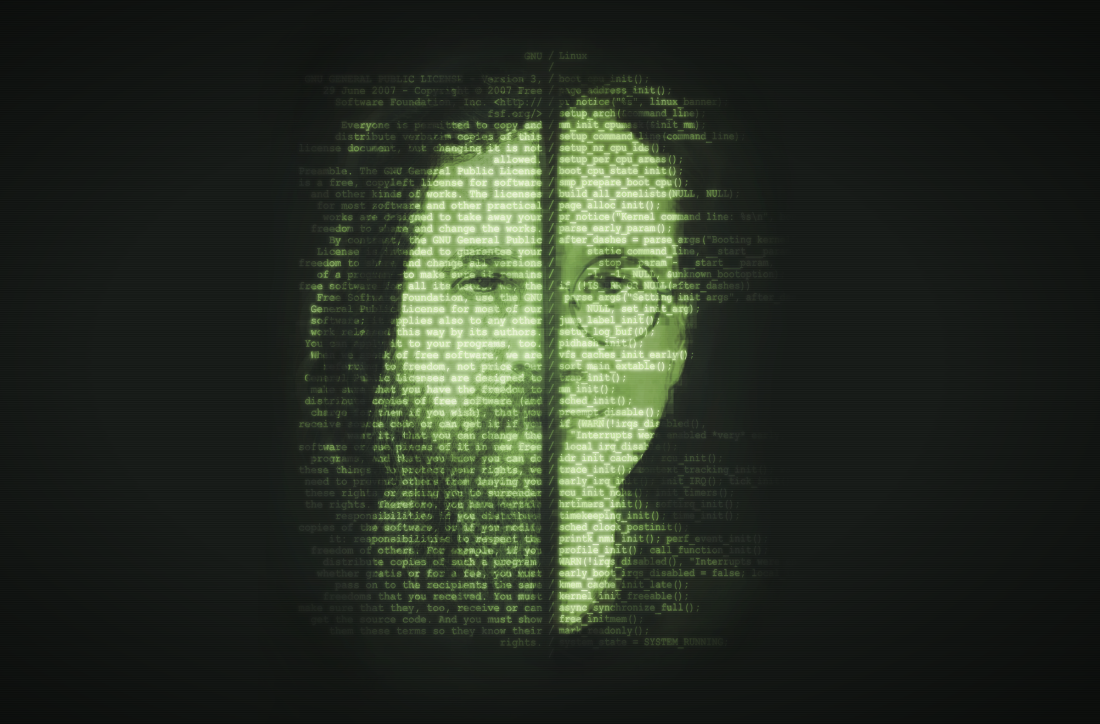
\includegraphics
   [height=\paperheight]{images/gnu-linux_wallpaper_tb_david_revoy.png}}
\begin{frame}[plain]%{LT}
%  
\note{GNU/Linux}
\end{frame}
\setbeamertemplate{background canvas}{}

\begin{frame}{Communautés et structures du libre}

  \begin{block}{International}
    Free Software Fondation : \url{https://www.fsf.org/}

    Open Source Initiative : \url{https://opensource.org/}

    Linux Fondation : \url{https://www.linuxfoundation.org/}

    Communautés de développeurs par projets (debian, Ubuntu, python...)
  \end{block}

\pause

  \begin{block}{France}
    CNLL : \url{http://cnll.fr/}

    April : \url{https://april.org/}

    Framasoft : \url{https://framasoft.org/}

    Toulibre : \url{http://toulibre.org/}

    etc...
  \end{block}
\end{frame}


\begin{frame}{Libre et/ou Opensource}

  \begin{block}{Libre}
    Mouvement social, question de liberté et de communauté. \textit{"Toutes les libertés dépendent de la liberté informatique, elle n’est pas plus importante que les autres libertés fondamentales mais, au fur et à mesure que les pratiques de la vie basculent sur l’ordinateur, on en aura besoin pour maintenir les autres libertés". (RMS)}
  \end{block}

  \begin{block}{Open-source}
    Open-source : code ouvert, méthodologie de développement, \textit{"l'idéologie, c'est nul"} (selon LT), pragmatisme
  \end{block}

On est toujours l'idéologue de quelqu'un... Débat dépassé ?
\end{frame}

\section{Vocabulaire}

\begin{frame}{Vocabulaire}

  \begin{itemize}
  \item \textbf{Logiciels privatifs} et non propriétaires (tous le sont !)
  \item \textbf{Copyleft} : \textit{droit laissé}, obligation de garantir que les libertés offertes par la licence soient préservées lors de la redistribution.
  \item \textbf{Copyright} : pas de valeur juridique particulière en France mais permet d'identifier les auteurs...
  \item Oeuvre : création originale, pas vraiment de sens dans le monde numérique
  \item Originalité : expression juridique de la créativité de l'auteur, empreinte de sa personnalité. \textbf{Création intellectuelle} dans le monde numérique
  \end{itemize}
\end{frame}

\section{Droit d'auteur}

\begin{frame}{Droit d'auteur}

  \begin{itemize}
  \item Droits patrimoniaux
    \begin{itemize}
    \item Droit de reproduction, de représentation
    \item Droit de suite (pas pour les logiciels)
    \item Droits voisins
    \end{itemize}
  \item Droits extra-patrimoniaux
    \begin{itemize}
    \item perpétuels et inaliénables
    \item paternité, divulgation  respect de l'oeuvre, repentir, retrait (quasi éradication dans le numérique).
    \end{itemize}
  \end{itemize}

 \begin{alertblock}{Droit d'auteur adapté}
    Libre et privatif sont régis par le \textit{droit d'auteur adaptés au logiciels}.
  \end{alertblock}

  \begin{alertblock}{Gauche d'auteur}
    Le libre est adossé au droit d'auteur.
  \end{alertblock}
  
  Les idées sont de libre parcours.
\end{frame}

%%%%%%%%%%%%%%%%%%%%%%%%%%%%%%%%%%%%%%%%%%%%%%%%%%%%%%%%
% Logiciel privatif
%%%%%%%%%%%%%%%%%%%%%%%%%%%%%%%%%%%%%%%%%%%%%%%%%%%%%%%%

\section{Privatif}


\begin{frame}{Logiciels privatifs}
  Principe général : réserver l'intégralité des droits au titulaire. Droits patrimoniaux organisés pour assurer un monopole d'exploitation économique.

  \begin{alertblock}{Définition : logiciel privatif}
    Logiciel sous licence privative, c'est-à-dire n'offrant pas au moins une des quatre libertés des licences libres.    
  \end{alertblock}

\pause

  \begin{block}{Michel Rocard, 2002, bataille des brevets : 648 contre, 14 pour, 18 abs}
   \textit{ La création, la liberté, l'innovation étaient du côté des logiciels libres. La recherche du profit et surtout la rente, le souci de freiner la concurrence et d'étouffer le buissonnement extérieur étaient du côté de la grosse industrie.
}
  \end{block}
\end{frame}

\begin{frame}{Gouvernance ?}
  
\textit{Si on ne peut pas rentrer par la porte, rentrons par la fenêtre !}

Qui gouverne quel projet de logiciel libre ? Posez-vous juste la question.

\end{frame}


%%%%%%%%%%%%%%%%%%%%%%%%%%%%%%%%%%%%%%%%%%%%%%%%%%%%%%%%
% Logiciel libre : 4 libertés
%%%%%%%%%%%%%%%%%%%%%%%%%%%%%%%%%%%%%%%%%%%%%%%%%%%%%%%%

\section{Libre}

\begin{frame}{logiciels libres}

  \begin{alertblock}{Principe général}
    Toutes les licences entendent que le \textit{code source} reste libre.
  \end{alertblock}
  Elles ne divergent principalement que sur les modalités de redistribution :
  \begin{itemize}
  \item pas d'obligation de redistribuer le code
  \item obligation de redistribuer le code sous les mêmes termes : empêcher de tirer bénéfice du logiciel sans reverser en retour sa propre oeuvre dérivée.
  \end{itemize}

  \begin{alertblock}{Définition : logiciel libre}
    Logiciel sous licence libre, c'est-à-dire offrant les quatre libertés des licences libres.    
  \end{alertblock}
  
\end{frame}



\begin{frame}{liberté 0 : liberté d'utilisation}
  \begin{itemize}
  \item Absolue liberté d'utilisation sans aucune restriction
  \item Oeuvre produite en utilisant un logiciel libre n'est pas soumise à sa licence
  \item Résultats produits par un logiciel : parfois des oeuvres dérivées...
  \item Quid de l'utilisation sans distribution ?
  \end{itemize}

  \begin{alertblock}{Principe}
    Dans l'intérêt du licencié.
  \end{alertblock}
  
  Question rapide : Est-ce que la licence de JSON est libre ? \url{http://www.json.org/license.html}

\end{frame}


\begin{frame}{liberté 1 : liberté d'étude}
  \begin{itemize}
  \item Liberté d'étude : aucun obstacle juridique ou technique.
  \item Pas obligatoire de livrer le source avec le binaire (=pragmatisme)
  \item Mise à disposition des sources à cout nul ou faible
  \item Code source mis à diposition au minium 3 ans (GPLv3)
  \end{itemize}
  \begin{alertblock}{Principe}
    Dans l'intérêt du licencié encore.
  \end{alertblock}
\end{frame}


\begin{frame}{liberté 2 : liberté de modification}
  \begin{itemize}
  \item Liberté de modification absolue mais restriction si distribution
  \item Préserver les mentions de titularité du droit d'auteur
  \item Droit au nom : identifier les contributeurs (L.121-1 du CPI) et même convention de Berne (internationalement reconnu)
  \item Droit au respect de la réputation mis en oeuvre par certaines licences : identifier les contributions.
  \end{itemize}
\begin{alertblock}{Principe}
    Dans l'intérêt du licencié toujours.
  \end{alertblock}
\end{frame}


\begin{frame}{liberté 3 : liberté de redistribution}
  \begin{itemize}
  \item Modalités de redistribution : principale différence entre licences libres :
    \begin{itemize}
    \item \textbf{Copyleft fort}
    \item \textbf{Copyleft faible}
    \item \textbf{Copyfree}
    \end{itemize}
  \item Droit au nom : identifier les contributeurs (L.121-1 du CPI et convention de Berne)
  \item Droit au respect de la réputation mis en oeuvre par certaines licences : identifier les contributions.
  \end{itemize}
\begin{alertblock}{Principe}
    Dans l'intérêt des autres utilisateurs. Cette liberté est surtout une condition nécessaire aux 3 précédentes.
  \end{alertblock}

\begin{alertblock}{Quand la licence se déclenchent-elles ?}
\textbf{Redistribuer déclenche la licence}
 \end{alertblock}
 
 Exception : AGPL où dès qu'il y a interaction avec le service, les obligation de la licence se déclenchent (art. 13)
\end{frame}

\section{TP1}

\begin{frame}{Étude des 4 "libertés" des logiciels privatifs}
  En 30 minutes et par groupe de 3 :
  \begin{itemize}
  \item ouvrir un pad collaboratif
  \item analyser pour chacune des 4 libertés du logiciel libre leur transposition dans les logiciels privatifs
  \item la mise en commun des travaux des groupes se fera sur un pad commun
  \end{itemize}

  \begin{alertblock}{Consigne générale}
    Toujours sourcer vos informations    
  \end{alertblock}
\end{frame}

\section{TP2}

\begin{frame}{Le libre dans vos entreprises ?}

  \begin{itemize}
  \item Y-a-t-il une "gouvernance" autour du libre dans vos
    entreprises ?
  \item Utilisez-vous des briques libres dans vos développements ? Précisez.
  \end{itemize}
Mise en commun sur :
\url{https://frama.link/entrepriseLL}
  
\end{frame}


%%%%%%%%%%%%%%%%%%%%%%%%%%%%%%%%%%%%%%%%%%%%%%%%%%%%%%%%
% Classification
%%%%%%%%%%%%%%%%%%%%%%%%%%%%%%%%%%%%%%%%%%%%%%%%%%%%%%%%


\section{Classification}


\begin{frame}{Licence diffusive}

  \begin{block}{Principe général}
    Empêcher de tirer bénéfice auprès de tiers sans reverser en retour sa propre contribution    
  \end{block}

  \begin{alertblock}{Définition (Pellegrini, Canevet)}
    Licence libre \textbf{avec copyleft} imposant que toute nouvelle contribution "s'appuyant" sur du code source placé sous cette licence soit également placé sous les termes de cette licence
   \end{alertblock}

On parle de \textit{\textbf{copyleft fort}}.

Autre termes rencontrés : "licences virales", "contaminantes" (à éviter, idéologie embarquée).
  
Exemples : GNU GPL, CeCILL(A)....

Stratégiquement \textbf{expansionnistes}.
\end{frame}


\begin{frame}{Licence persistante}

\begin{block}{Principe général}
    Empêcher toute privatisation de l'oeuvre sans s'appliquer aux oeuvres dérivées.
  \end{block}

  \begin{alertblock}{Définition (Pellegrini, Canevet)}
    Licence libre \textbf{avec copyleft} n'empêchant pas l'usage des oeuvres placées sous leur régime au sein d'oeuvres placées sous d'autres licences (y compris privatives)
   \end{alertblock}

On parle de \textit{\textbf{copyleft faible}}, licences "pérennes". Plutôt pour des librairies.
 
Exemples : GNU LGPL, CeCILL-C (Composant)

Stratégiquement \textbf{défensives}.

\end{frame}


\begin{frame}{Licence évanescente}
  \begin{block}{Principe général}
    Liberté totale !
  \end{block}

  \begin{alertblock}{Définition (Pellegrini, Canevet)}
    Licence libre \textbf{sans copyleft} autorisant la redistribution du logiciel sans son code source.
   \end{alertblock}

On parle de \textit{\textbf{copyfree}}

Autre terme moins rigoureux : licences permissives 

Exemples : BSD (BSD 4 clauses, BSD 3, BSD 2), MIT, Apache, CeCILL-B... 

Stratégiquement \textbf{prosélytes}.
\end{frame}


\section{Périmètre}


\begin{frame}{Comment s'appliquent les licences libres ?}
  \begin{alertblock}{Problématique}
    Comment se propagent les obligations de la licence pour une contribution donnée ? 
  \end{alertblock}

  \begin{block}{Idée générale}
    Respecter l'esprit de la licence initiale    
  \end{block}

  \begin{itemize}
  \item copyleft : préserver la liberté du code (plus ou moins strictement)
  \item copyfree : pas d'obligation de distribuer le source
  \end{itemize}

Même une diffusive n'a pas une propagation sans limites !
  
\end{frame}


\begin{frame}{Limites des diffusives}
La diffusivité n'est pas du tout absolue.

  \begin{block}{But général des diffusives}
    \begin{itemize}
    \item Contrepartie
    \item Coexistence
    \end{itemize}
  \end{block}

  \begin{itemize}
  \item Diffusivité ascendante si oeuvre dérivée (\textbf{\textit{basée}} sur celui-ci au sens du droit d'auteur). Bibliothèque et appels systèmes (libc LGPL et Linux GPLv2) ? 
  \item Diffusivité descendante : pilotes = oeuvre dérivée ? (wrapper)
  \end{itemize}

Oeuvre dérivée dès qu'il n'y pas substituabilité (selon si le couplage avec le code diffusif est spécifique ou générique)

  \begin{alertblock}{Périmètre}
    Le périmètre de la licence est défini par la substituabilité..
  \end{alertblock}
\end{frame}


\begin{frame}{Limites des persistantes}
Trois cas :
  \begin{itemize}
  \item oeuvre utilisant... : Si "oeuvre considérée comme utilisant simplement la bibliothèque", pas
    d'obligations (sauf liaison statique, voir licence)
  \item oeuvres combinées.... avec la bibliothèque
  \item ajout de fonctionnalités
  \end{itemize}

Préserver le périmètre fonctionnel du logiciel couvert pour éviter subversion... (cf MPL)

Périmètre défini de façon abstraite et fonctionnelle en termes de modules
 \begin{alertblock}{Périmètre}
    Le périmètre de la licence est l'interface.
  \end{alertblock}
  
\end{frame}


\begin{frame}{Utilisation des évanescentes}

  \begin{block}{But général des évanescentes}
    Aucune obligation de distribuer le source avec le code objet.
  \end{block}

  \begin{alertblock}{Périmètre}
    Le périmètre de la licence est le fichier lui-même.
  \end{alertblock}

  Suivre les indications des licences...

\end{frame}


%%%%%%%%%%%%%%%%%%%%%%%%%%%%%%%%%%%%%%%%%%%%%%%%%%%%%%%%
% Compatibilité
%%%%%%%%%%%%%%%%%%%%%%%%%%%%%%%%%%%%%%%%%%%%%%%%%%%%%%%%

\section{Compatibilité}


\begin{frame}{Quelles compatibilités entre licences libres ?}

  \begin{block}{Définition : licences incompatibles}
    Licences qui imposent des obligations contradictoires.. 
  \end{block}

  \begin{alertblock}{Licence B est compatible avec licence A si :}
    \begin{itemize}
    \item les droits de B sont inclus dans ceux de A
    \item les obligations de A sont incluses dans celles de B
    \end{itemize}
  \end{alertblock}

\pause

\begin{alertblock}{\textit{nemo plus juris}}
  \textit{Personne ne peut transférer à autrui plus de droits qu'il n'en a lui-même.}
\end{alertblock}

Les licences diffusives sont par nature incompatibles entre elles...

\end{frame}


\begin{frame}{La compatibilité en un tableau}

Votre code = du code + A + B. Pouvez-vous le distribuer ?


\scalebox{0.7}{
  \begin{tabularx}{14cm}{|X|X|X|X|}
    \hline
\backslashbox{Code A}{Code B}   & Diffusive & Persistante & Evanescente \\
\hline
Diffusive & \textbf{Impossible} sauf si clause de compatibilité & \textbf{Impossible} sauf si clause de compatibilité & \textbf{Possible} P peut être distribué sous la licence de A\\
\hline
Persistante& \textbf{Impossible} sauf si clause de compatibilité & \textbf{Possible}. Distribution sans que les licences A et B ne se diffusent et à condition que chaque module soit distribué sous sa propre licence  & \textbf{Possible}. Distribution sans que la licence de A ne se diffuse à la partie hachurée et au code B et à condition que A soit distribué sous sa licence. \\
\hline
Evanescente & \textbf{Possible}. P peut être distribué sous la licence B  & \textbf{Possible}. P peut être distribué sans que la licence B ne se diffuse à la partie hachurée et le module A à condition que B soit distribué sous la licence B & \textbf{Possible}. Aucune diffusivité. \\
\hline  
  \end{tabularx}
}
\end{frame}


\section{TP3 et TP4}


\begin{frame}{Lecture et analyse de licences}

Indispensable pour tout développeur au risque de râter sa vie.

\textit{The SMOG grade is a measure of readability that estimates the years of education needed to understand a piece of writing. SMOG is an acronym for Simple Measure of Gobbledygook.}

Selon Alexios Zavras, le SMOG grade moyen est de 17. Certaines licences dépassent 25.

\end{frame}


\begin{frame}{GPLv3}
  Par groupe de 3, dans le document fourni, lire et commenter la GPLv3 (durée 1h) :
  \begin{itemize}
    \item reformuler clairement sans paraphraser
    \item expliquer en détail certaines notions : pourquoi sont-elles introduites, approfondir (brevets, MTP, diffusivité...)
    \item comparer même brièvement avec d'autres licences libres (CeCILL, MIT, LGPL, AGPL...)
   \end{itemize}

  \begin{center}
    \includegraphics[width=0.3\textwidth]{images/gplv3.png}
\end{center}
\end{frame}


\begin{frame}{3 questions}
 Par groupe de 3, répondez aux 3 questions tirées au sort
 \begin{itemize}
 \item Chaque groupe présentera ces réponses en 10 minutes
   questions de la promo comprises
 \item Notation en 7, 10, 12, 14, 18, 20.
 \end{itemize}
\end{frame}


%%%%%%%%%%%%%%%%%%%%%%%%%%%%%%%%%%%%%%%%%%%%%%%%%%%%%%%%
% Bonnes pratiques et audits
%%%%%%%%%%%%%%%%%%%%%%%%%%%%%%%%%%%%%%%%%%%%%%%%%%%%%%%%

\section{Bonnes pratiques et audits}


\begin{frame}{Bonnes pratiques}
  \begin{itemize}
  \item Ne pas supprimer les mentions de copyright !
  \item Gérer la diffusivité
  \item Respecter le formalisme de chaque licence
  \item Se soucier dès le début du projet et tout au long de celui-ci de la faisabilité juridique !
  \item Pas uniquement des juristes... Besoin de personnes avec connaissances techniques (profil rare)
  \end{itemize}
Sinon :
\begin{itemize}
\item réécrire (en moins bien) des modules en urgence
\item retards dans la livraison
\item violation de licence (procédures, image de la société, impact sur les clients...)
\end{itemize}
\end{frame}


\begin{frame}{Audits, pourquoi ?}

Selon \textit{Black Duck Software} :
\begin{itemize}
\item 30\% de la base de code des entreprises serait libre
\item 98\% des entreprises ne le sauraient pas...

\end{itemize}
\begin{minipage}[c]{0.4\linewidth}
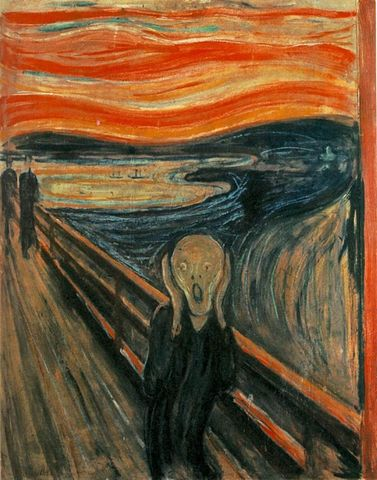
\includegraphics[width=0.9\textwidth]{images/The_Scream.jpg}\end{minipage}
\begin{minipage}[c]{0.5\linewidth}
Marketing de la \textit{peur} mais :

Double contrainte :
\begin{itemize}
\item juridique : compatibilité des licences (privatives, libres, libres entre elles
\item technique : failles de sécurités de n'importe quel composant externes (HeartBleed dans OpenSSL, ...)
\end{itemize}
\end{minipage}
Finalement, une chance que les composants impactés soient des logiciels libres...
  
\end{frame}

\subsection{Outils}

\begin{frame}{Audits, comment ?}

Essentiellement trois solutions...

\end{frame}

%%%%%%%%%%%
% BlackDuck
%%%%%%%%%%%%

\begin{frame}{BlackDuck}
  Fondé par un ancien de Microsoft.

  \begin{itemize}
  \item Open Source Application Security
  \item Open Source Compliance and Management
  \end{itemize}

\url{https://www.blackducksoftware.com/}
\end{frame}

%%%%%%%%%%%
% FOSSology
%%%%%%%%%%%%


\begin{frame}{FOSSology}
\begin{block}{FOSSology}
\textit{License compliance software system and toolkit.}
\end{block}
\begin{itemize}
\item \textit{As a toolkit you can run license, copyright and export control scans from the command line.}
\item textit{As a system, a database and web ui are provided to give you a compliance workflow. License, copyright and export scanners are tools available to help with your compliance activities.}
\end{itemize}
\url{https://github.com/fossology/fossology}
\end{frame}


\setbeamertemplate{background canvas}{\centering\includegraphics
   [height=\paperheight]{images/fossology-linux-kernel.png}}
\begin{frame}[plain]%{RMS}
%  
\note{RMS}
\end{frame}
\setbeamertemplate{background canvas}{}


%%%%%%%%%%%
% Scancode toolkit
%%%%%%%%%%%%

\begin{frame}{Scancode toolkit}
\textit{ ScanCode is a suite of utilities used to scan a codebase for license, copyright, and other interesting information that can be discovered in files.}

\textit{A typical software project often reuses hundreds of third-party components. License and origin information is often scattered and not easy to find: ScanCode discovers this data for you.}

\url{https://github.com/nexB/scancode-toolkit}
\end{frame}

\setbeamertemplate{background canvas}{\centering\includegraphics
   [width=\paperwidth]{images/scancode-ffmpeg.png}}
\begin{frame}[plain]%{RMS}
%  
\note{RMS}
\end{frame}
\setbeamertemplate{background canvas}{}


%%%%%%%%%%%%%%%%%%%%%%%%%%%%%%%%%%%%%%%%%%%%%%%%%%%%%%%%
% Futur
%%%%%%%%%%%%%%%%%%%%%%%%%%%%%%%%%%%%%%%%%%%%%%%%%%%%%%%%

\section{Futur ?}

\begin{frame}{Licences à réciprocité}

Préliminaire : avoir des juristes compétents sur ces thèmes.

  \begin{block}{Problèmes}
    \begin{itemize}
    \item 70\% des contributions à Linux proviennent de quelques entreprises. Lesquelles ?
    \item Wikipédia dépend fortement de Google.
    \item ....
    \item Gouvernance communautaire ? 
    \end{itemize}
  \end{block}

  \begin{block}{Pistes}
    \begin{itemize}
    \item "Peer Production Licence" \textit{(copyfarleft})
    \item "Commons reciprocity licence"
    \item "Fair source"
    \item Licence = mauvaise piste ? Piste légale plutôt ?
    \end{itemize}
  
  \end{block}
  
Voir conférence de Calimaq : \url{https://scinfolex.com/tag/capitole-du-libre/}
  
\end{frame}

\section{Bibliographie et crédits}

\begin{frame}{Bibliographie/Webographie}

Bibliographie :

  \begin{itemize}
  \item "Droit des logiciels, logiciels privatifs, logiciels libres", F.Pellegrini et S.Canevet, PUF 2013.
  \item "Option libre. Du bon usage des licences libres", B.Jean, Framabook 2012.
  \item "Histoire et cultures du Libre. Des logiciels partagés aux licences partagés", Collectif, Framabook 2013.
  \end{itemize}

Webographie :

\begin{itemize}
\item \url{http://gplv3.fsf.org/}
\item \url{https://linuxfr.org/}
\item \url{http://april.org/}
\end{itemize}
  
\end{frame}

\begin{frame}{Crédits 1/2}
  \begin{itemize}
  \item Photo de Richard Stallman par Lionel Allorge, licence GFDL1.3+, CC-BY-SA+, LAL+,  \url{http://photos.april.org/picture.php?/4413/category/159}
  \item Photo de Linus Torvalds de Wikimédia Commons, licence CC-BY-SA 3.0 capture d'une vidéo de Linux Foundation Kernel Summit 2008 \url{https://upload.wikimedia.org/wikipedia/commons/3/31/Linus_Torvalds_lks08.jpg}
  \item GNU/Linux, David Revoy, CC-BY \url{http://deevad.deviantart.com/art/GNU-Linux-Portrait-645635708}
   \end{itemize}
\end{frame}


\begin{frame}{Crédits 2/2}
  \begin{itemize}
\item SMOG grade : Zavras, Alexios (2016) ‘Twenty-five years of school? Analysis of Free and Open Source software license texts’, International Free and Open Source Software Law Review, 8(1),
pp 29 – 44 DOI: 10.5033/ifosslr.v8i1.111  
\item Logo GPLv3, licence GFDL : \url{http://www.gnu.org/graphics/license-logos.html}
\item The Scream by Edward Munch, Public domain : \url{https://commons.wikimedia.org/wiki/File:The_Scream.jpg}

  \end{itemize}
\end{frame}



\begin{frame}{Licence}
  Document sous licence GFDL1.3+, CC-BY-SA+, LAL+.
\end{frame}



\end{document}
